\documentclass[12pt,a4paper]{article}
%\usepackage[utf8]{inputenc}
%\usepackage[hidelinks]{hyperref}
\usepackage{caption}
\usepackage{hyperref}
\usepackage{cite}
\usepackage[version=4]{mhchem} % for isotope symbols
\usepackage{a4wide}
\usepackage[lmargin=2cm,rmargin=2cm,tmargin=2cm,bmargin=2cm,headheight=0in]{geometry}
\usepackage{amssymb}
\usepackage{graphicx}


%\hypersetup{colorlinks, linkcolor={blue!50!black}, citecolor={blue!50!black},
%	urlcolor={blue!50!black}}
	
% Caption font sizes	
\DeclareCaptionFont{CaptionFontSize}{\fontsize{12pt}{12pt}}
\captionsetup[table]{font=CaptionFontSize}
\captionsetup[figure]{font=CaptionFontSize}

%Making bibliography compact
\let\oldbibliography\thebibliography
\renewcommand{\thebibliography}[1]{\oldbibliography{#1}
\setlength{\itemsep}{0pt}
\setlength{\parskip}{0pt}}

%\renewcommand{\bibliographytypesize}{\fontsize{10pt}{10pt}}

\newcommand{\cdm}{\ce{^{113\text{m}}Cd}}

\begin{document}
%\title{Nuclear isomers for energy storage and fundamental physics} - broad
%\title{Investigation of the energy storage potential of $\ce{^{113m}Cd}$ using time-correlated gamma ray-coincidence spectroscopy}% - narrower
%\title{Investigation of $\ce^{{113m}Cd}$ for energy storage and the physics of breakup in nuclear reactions} - narrowest
%\title{Investigation of $\ce{^{148,150,152}Ce}$ and $\ce{^{113m}Cd}$ using time-correlated gamma ray-coincidence spectroscopy}
%\title{Searching for octupole collectivity in neutron-rich Ce isotopes and isomer depletion pathways in $\ce{^{113}Cd}$} % Working title
%\author{Student: Caspian Nicholls (u1027945)}
%\date{Supervisor: Dr. A. J. Mitchell, Department of Nuclear Physics, Research School of Physics and Engineering, Australian National University}
%\date{\today}

\noindent
\textbf{Title: }Searching for octupole collectivity in neutron-rich Ce isotopes and isomer depletion pathways in $\ce{^{113}Cd}$

\noindent
\textbf{Author: } Caspian Nicholls (u1027945)

\noindent
\textbf{Supervisor: } Dr. A. J. Mitchell, Department of Nuclear Physics, Research School of Physics and Engineering, Australian National University

% From AJ
%Title: Probably needs to change. Something like “Search for octupole collectivity in neutron-rich Ce isotopes and isomer depletion pathways in 113Cd” ? 
%
%Context and aims: Opening paragraph to explain the situation of project change, then broader context. Set out the timeline of La decay analysis now until end of June. Reassess. Cd experiment ~ August (?) if possible. If this is set out clearly, then the rest can follow more easily. 
%

\section*{Context and Aims}

Gamma-ray spectroscopy is a powerful tool for studying the internal structure of atomic nuclei.
This project initially revolved around using this technique to investigate energy storage and release mechanisms of an excited metastable state of $\ce{^{113}Cd}$ with an exceptionally long half-life, known as a \textit{nuclear isomer}.
However, due to the global COVID-19 outbreak, the ANU Heavy Ion Accelerator Facility (HIAF) has been closed until June 26$^\text{th}$.
Consequently, experiments that were planned for this project have been postponed.
Assuming the HIAF reopens as planned with enough time to perform these experiments and thoroughly analyse the resulting data, the aim is to return to this line of research.
In the interim, this project will focus on analysing yet unstudied experimental data on exotic, neutron-rich cerium isotopes.

\medskip
\noindent
Primarily, nuclear isomers are worth investigating for energy storage applications because nuclei store around $10^9$ J/g of harnessable energy, approximately four orders of magnitude greater than the fundamental chemical limit of conventional fuels.
Hence, isomers with decay half-lives greater than one year are currently being methodically studied to establish their suitability for use in long-term energy storage devices.
These devices would suit use in highly remote or largely inaccessible areas, where regularly restocking energy supplies may be impractical or inefficient~\cite{shaffer_innovations_2018}.

\medskip
\noindent
One such long-lived isomer (denoted $\cdm$) exists in $\ce{^{113}Cd}$ with a half-life $T_{1/2} = 14.1$~years and excitation energy of 264~keV, making it a worthwhile candidate for such applications.
However, realising the potential of this metastable requires finding a mechanism by which its energy can be released.
A current frontrunner is \textit{isomer depletion}, where a nuclear isomer is excited into a more energetic \textit{intermediate state} (or \textit{depletion level}) that can then rapidly decay via a sequence of gamma-ray transitions (\textit{depletion pathway}) into the ground state.
Isomer depletion has been investigated for metastable states of a small number of other isotopes, but not yet for $\cdm$~\cite{shaffer_innovations_2018}.

\medskip
\noindent
This project would be centered around constructing a picture of the excited states (\textit{level scheme}) of $\ce{^{113}Cd}$ and finding favourable depletion pathways that connect the isomer to the ground state.
Excited states in $\ce{^{113}Cd}$ would be populated through break-up/fusion-evaporation nuclear reactions, induced by an accelerated ion beam delivered by the 14UD tandem accelerator at the HIAF.
In fusion-evaporation reactions, beam and target fuse to produce a compound nucleus that preferentially emits particles (typically p, n or $\alpha$) over gamma rays, due to its significant excitation energy.
Different combinations of massive particles can be emitted: one of these \textit{reaction channels} will yield excited states of $\ce{^{113}Cd}$.

\medskip
\noindent
Excited states of $\ce{^{113}Cd}$ can also be produced via break-up reactions, where the beam particle separates into smaller fragments.
These reactions have been experimentally observed, occurring when one of the beam fragments has the right nucleonic content to react with the target and produce an excited form of the isotope of interest~\cite{curtis_+li_2005,dasgupta_fusion_1999}. 
%, such as $\ce{^{7}_{3}Li} \rightarrow \ce{^{4}_{2}\alpha} + \ce{^{3}_{1}t}$ (t: tritium).
Irrespective of how excited $\ce{^{113}Cd}$ nuclei are formed, the CAESAR array of High-Purity Ge (HPGe) detectors will measure the gamma rays that depopulate these excited states.


\medskip
\noindent
Whilst these experiments are infeasible, existing data on the isotopes $\ce{^{148,150,152}Ce}$ will be analysed to test a prediction of the deformed shell model of nuclear structure: that charge distributions of nuclides with proton numbers $Z$ near 56 and neutron numbers $N$ near 88 can take on reflection-asymmetric pear-like shapes.
In $\ce{^{148,150,152}Ce}$, these deviations from sphericity are induced by dynamic octupole deformation, due to the collective motion (\textit{octupole collectivity}) that occurs when a nucleus undergoes octupole vibrations.
In other nuclides, these shapes can arise from a permanent, static octupole deformation of the ground state due to its nucleonic configuration~\cite{butler_intrinsic_1996}.
%These shapes arise from octupole deformation, a phenomenon that can have either a dynamic (due to specific vibrations of an excited state) or static shape (corresponding to a permanent deformation of the ground state).


\medskip
\noindent
Octupole deformations are relatively rare amongst nuclides: spherical, quadrupole-prolate deformed (upright-rugby-ball) and quadrupole-oblate deformed (discus) shapes are most prevalent.
Yet, they are still worth studying: nuclei with permanent octupole deformations could have permanent non-zero atomic electric-dipole moments, the observation of which would suggest charge-parity violation due to physics beyond the standard model~\cite{gaffney_studies_2013}.
Strong octupole correlations are expected in nuclides with similar nucleonic content to $\ce{^{224}Ra}$ and $\ce{^{146}Ba}$, including $\ce{^{148,150,152}Ce}$~\cite{bucher_direct_2017}.
As these nuclides contain large numbers of nucleons, the fact the octupole collectivity they exhibit can be described in terms of particular interactions between a small number of nucleon pairs is worth understanding~\cite{casten_nuclear_1990}.
%% Is it the charge distributions, nuclear density distributions or both that deviate from spherical?

\medskip
\noindent
However, evidence for octupole deformation has only been observed for $\ce{^{220}Rn}$, $\ce{^{224}Ra}$ and $\ce{^{144,146}Ba}$~\cite{bucher_direct_2017,bucher_direct_2016}.
By studying $\ce{^{148,150,152}Ce}$, the primary research aim of this project is to generate new information on the collective motion that occurs during low-energy octupole vibrations.

\medskip
\noindent
To achieve this, recorded data on the gamma rays emitted by excited states of $\ce{^{148,150,152}Ce}$ will be analysed.
Specifically, a level scheme for these nuclides will be constructed, including spectroscopic data (excitation energies, lifetimes, spins and parities) for the low-lying excited states.
Using this information, dipole and quadrupole moments of the charge distribution of the nuclei will be determined, which will in turn enable the octupole collectivity of these isotopes to be quantified.

\medskip
\noindent
A common goal of these research aims is to develop and utilise gamma-ray spectroscopic analysis routines to extract key information from multi-parameter nuclear data, then meaningfully interpret this data in the context of various theoretical nuclear structure models.

\medskip
\noindent
The latter aim above ties in with ongoing work to test predictions made by theoretical nuclear structure models and further our understanding of nuclear physics.
An understanding of this field has useful applications in energy storage~\cite{shaffer_innovations_2018}, astrophysics~\cite{hayakawa_neutron_2009}, nuclear medicine~\cite{krane_introductory_1987}, relativity and particle physics~\cite{casten_nuclear_1990}.

\section*{Background}

\subsection*{Octupole collectivity}

\medskip
\noindent
Atomic nuclei are complicated collections of quantum objects.
According to the shell model of nuclear structure, protons and neutrons independently fill sets of orbitals.
The binding energies of these orbitals are irregularly distributed, yet, inclusion of the spin-orbit interaction in the nuclear Hamiltonian results in the emergence of magic numbers akin to those for electron shells.
Magic numbers of protons or neutrons form closed shells of filled orbits, which remain unchanged when the nucleus they reside in is excited.
As a result, the behaviour of a few valence nucleons can govern the character of nearly magic nuclei: those with $Z$ and $N$ near magic numbers.
Often, they are said to occupy \textit{single-particle states}, since the state of the nucleus can be described by considering just the motion of a single nucleon between orbitals.

\medskip
\noindent
As $N$ and $Z$ move away from these magic numbers, nuclei gradually shift away from sphericity.
The behaviour of these mid-shell nuclei is commonly modelled through considering rotations and vibrations of non-spherical nuclear shapes.
These motions are collective, since most (if not all) of the nucleons are involved.
This directly contrasts with the single-particle description of nearly magic nuclei~\cite{casten_nuclear_1990}.

\medskip
\noindent
The octupole vibrations that cause octupole collectivity correspond to a nuclear state that is a superposition of particle-hole excitations of angular momentum $3\hbar$ and negative parity: the recoupling of nucleons that have left their ground state orbitals is responsible for this excited nuclear state~\cite{rohozinski_octupole_1988}.
Specifically, the nucleons that recouple must occupy pairs of orbitals that lie near the outermost ground state valence orbital, have opposite parity, $\Delta n = 1$ and $\Delta l = \Delta j = 3$, so that these orbitals can be strongly coupled by the octupole interaction~\cite{butler_intrinsic_1996}.
Here, $n$, $l$ and $j$ denote the principal, orbital angular momentum and total angular momentum quantum numbers.

\medskip
\noindent
Octupole collectivity in nuclides near $\ce{^{146}_{56}Ba_{90}}$ can be described by considering the interaction of only a few nucleons because these nuclides lie just outside the $Z = 50$ and $N = 82$ shell closures.
For this behaviour to occur at low energies, the orbitals coupled by the octupole interaction must have only a small separation in energy.
Based on the deformed shell model, near $\ce{^{146}Ba}$, this \textit{octupole coupling}/\textit{correlation} is expected to be strongest between the $h_{11/2}$ and $d_{5/2}$ proton orbitals or the $i_{13/2}$ and $f_{7/2}$ neutron orbitals.

\medskip
\noindent
However, nuclei with strong octupole collectivity are difficult to study because they are hard to produce, being neutron rich and radioactive.
Early studies using HPGe arrays were limited to prompt fission spectroscopy, % using large HPGe arrays,
which typically only provides information on high-spin excited states.
More recently, the development of radioactive ion beams enabled Coulomb excitation experiments
%Large arrays of gamma ray detectors have been used to record the gamma rays emitted by high spin excited states of neutron-rich nuclei  near $\ce{^{144}Ba}$ (Z $\sim$ 56, N $\sim$ 88) (formed from the spontaneous fission of $\ce{^{252}Cf}$) and study octupole collectivity~\cite{phillips_octupole_1988,chen_search_2006}.
%Specifically, the observation of strong E1 transitions between the yrast energy levels - those lowest in energy for a given total angular momentum - has provided much of the experimental evidence for octupole correlations near $\ce{^{144}Ba}$~\cite{casten_nuclear_1990}.
to measure the octupole collectivity in $\ce{^{144,146}Ba}$.
These found that the strength of the octupole collectivity was significantly greater than theoretically predicted, suggesting that current models of nuclear structure may need to be revised~\cite{bucher_direct_2016,bucher_direct_2017}.
% Weisskopf strength that is: Weisskopf estimate much greater than 1 Weisskopf unit means that many particles participate in the transition between the ground state and the state corresponding to octupole vibration, so the motion (vibration) of the nucleus when it occupies that state is collective.

\medskip
\noindent
A more recent experiment at the CAlifornium Rare Ion Breeder Upgrade (CARIBU) facility at Argonne National Laboratory added 31 new excited states to the level scheme of $\ce{^{146}Ba}$, extending it up to $\sim2.5$~MeV.
To obtain these results, the $\beta^-$ decay of an accelerated beam of $\ce{^{146}Cs}$ extracted from the %(spontaneous)
fission of a $\ce{^{252}Cf}$ source was measured using a HPGe array~\cite{mitchell__2016}.
%
%\medskip
%\noindent
%Yet, relatively few studies of the neighbouring isotopes $\ce{^{148,150,152}Ce}$ have occurred. All their existing level schemes have come from measuring products of the spontaneous fission of $\ce{^{252}Cf}$~\cite{nica_notitle_117,
%martin_notitle_114,
%bazu_notitle_114}.

\medskip
\noindent
The data for this project was also generated at CARIBU by accelerating beams of $\ce{^{148,150,152}La}$ from the fission of $\ce{^{252}Cf}$.
The $\beta^-$ decay of each of these beams was then measured to obtain information on the low-spin states of $\ce{^{148,150,152}Ce}$, using a gamma-ray detector array (as done for $\ce{^{142,144,146}Ba}$~\cite{mach_influence_1990}). 
The accelerated beam particles were implanted onto a moving tape system, found at the target position of the detector array.
This system was used to periodically remove any sources with a long-lived activity that could have obscured the signals of interest~\cite{mitchell_x-array_2014}.

\medskip
\noindent
The detector array used contained four clover detectors (each accommodating four Ge detectors) and five fast-timing LaBr3(Ce) detectors.
A plastic scintillator detector was also included to detect $\beta^-$ particles.
These three detector types enable three-fold $\beta$-$\gamma$-$\gamma$ coincidence measurements to be made, which in turn allow specific excited states to be identified and their lifetimes measured.
The timing characteristics of the scintillator and LaBr(Ce) detectors used mean that this set up may enable measurement of excited state lifetimes as short as 30~ps.
These capabilities of the equipment used will thus enable the existing spectroscopic knowledge surrounding $\ce{^{148,150,152}Ce}$ to be expanded upon.

\subsection*{Nuclear isomers}
In general, nuclear isomers exist because their decay into less-excited states is inhibited.
This could be due to the fundamental quantum-mechanical selection rules preventing the isomer from easily decaying into any lower-energy states.
Otherwise, this inhibition can arise when the metastable state may only decay into states of vastly different total angular momentum $J$.
Transitions where the nucleus undergoes a large change in $J$ are slower; this change $\Delta J$ is the transition's \textit{multipolarity}.
Figure~\ref{fig:cd113} shows that $\cdm$ ($J^\pi = 11/2^-$, 263.54 keV) can only de-excite into the ground state ($J^\pi = 1/2^+$).
Thus it can only decay via an E5 transition with a relatively high multipolarity $\Delta J = 5\hbar$~\cite{blachot_notitle_111}; the E5 label refers to the spatial distribution of the emitted radiation,  which is governed by the transition multipolarity and the product of the initial and final parities ($\pi_i\pi_f = -1$).
\begin{figure}[htbp]
	\centering
	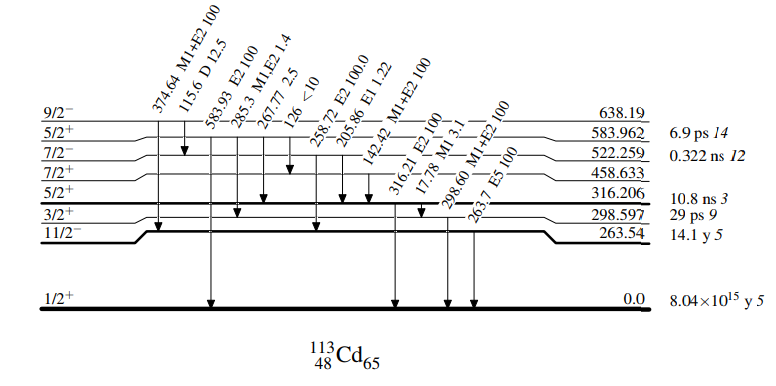
\includegraphics[width=0.9\textwidth]{113cd_partial_level_scheme_ENSDF.png}
	\caption{Partial level scheme for $\ce{^{113}Cd}$. The key isomeric state has an energy of 263.54~keV~\cite{blachot_notitle_111}, although another isomer is present at 316.206~keV.}
\label{fig:cd113}
\end{figure}

\medskip
\noindent
Figure~\ref{fig:cd113} suggests that there are pathways by which $\cdm$ could be excited into a more energetic state and then decay rapidly into the ground state.
For example, the isomer could be excited into the $7/2^-$ state at 522.259~keV, before releasing its 263.54~keV of stored energy by decaying to the ground state, via the 316.206-keV state.
However, decay back into the isomer is much more strongly favoured than this pathway, making it an unreliable option for isomer depletion.
Small changes in energy and large changes in either multipolarity or nucleonic configurations can inhibit transitions.
The first two do not apply to the depletion pathways in Figure~\ref{fig:cd113}, so the latter is likely why they are all unfavourable (confirming this would require identifying the orbital structure of $\ce{^{113}Cd}$ to associate  a nucleonic configuration with each state). % slide 12 of Greg L26 from PHYS3105
% decays can be inhibited due to the overlap between the parent and daughter wavefunctions being small


\medskip
\noindent
The feasibility of isomer depletion for energy-storage applications has been experimentally studied for six other nuclides ($\ce{^{180}Ta}$, $\ce{^{68}Cu}$, $\ce{^{177}Lu}$, $\ce{^{178}Hf}$, $\ce{^{108}Ag}$ and $\ce{^{93}Mo}$), using several distinct mechanisms.
These include exposing a sample containing a significant isomer population to bremsstrahlung radiation, using Coulomb excitation by accelerating ion beams, or initiating nuclear excitation by electron capture
~\cite{shaffer_innovations_2018}.
Identification of a favourable depletion pathway within $\ce{^{113}Cd}$ would thus extend the list of nuclides that may be harnessed to store energy over long timescales.
%Thus, should a practical depletion pathway be found within $\ce{^{113}Cd}$, these methods could be explored to demonstrate isomer depletion within this nuclide.
% Description of relevant models? Shell model, Nilsson/deformed shell model, ...?

\section*{Project Description}

\medskip
\noindent
The analysis techniques and software that will be used are all well documented and commonly used by my research group, so a wealth of knowledge can be readily consulted whenever data processing queries arise.
$\ce{^{148}Ce}$ and $\ce{^{150}Ce}$ have been studied using La $\beta^-$ decay experiments.
Analysing the recorded data for these isotopes will build on existing knowledge, extend level schemes and potentially verify currently-tentative spin-parity assignments.
Contrastingly, $\ce{^{152}Ce}$ has only been studied via the spontaneous fission of $\ce{^{252}Cf}$, so inspecting the $\beta^-$ decay data of $\ce{^{152}La}$ should provide new information on its structure.
Ultimately, however, dedicated octupole collectivity studies have not been performed for any of these Ce isotopes, so this project will be breaking new ground.
% Too grandiose?

\medskip
\noindent
To produce the results described above, $\beta$-$\gamma$ and $\beta$-$\gamma$-$\gamma$ coincidence analysis methods will be implemented in the data analysis framework ROOT and the Radware suite.
These coincidence methods rely on multiple particles being detected by different detectors in a time window that is narrow enough to conclude they came from the same nucleus.
The consideration of $\gamma$-$\gamma$ coincidences (from the clover detectors) where one of the $\gamma$ rays is known to be emitted by a Ce isotope will also be vital.
Further analysis of gamma-ray spectra will then lead to the collection of key spectroscopic information, including state lifetimes, excitation energies and spin-parities. %how for spin-parities?

\medskip
\noindent
Evidence for octupole collectivity will then be identified through classifying strong E1 transitions between yrast bands of opposite parity.
This will require of the identification of the yrast bands, which have the least excitation energy for a given $J$~\cite{casten_nuclear_1990}.
% How do we identify the yrast bands?
The degree to which octupole collectivity occurs in each Ce isotope will then be assessed by evaluating the dipole and quadrupole moments of different transitions.
% These moments can be identified from the decay rate (1/state lifetime?) -  see Greg L26 from PHYS3105

% Be sure to justify the methods chosen more clearly, and explain how this work fits into the field. This also holds for the octupole collectivity part - done for now.
% Need to highlight that the octupole collectivity stuff is new/original (based on the research proposal for the experiments themselves) whilst the cadmium stuff is largely just trying to build on what has been done before - done for now.

\medskip
\noindent
As for the nuclear isomer side of this project, existing knowledge of the level scheme of $\ce{^{113}Cd}$ will be expanded upon.
Some preparatory work for this phase has already occurred (Figure~\ref{fig:gantt}), including reviewing previous experiments that studied excited states of $\ce{^{113}Cd}$.
The qualitative behaviour of the relevant reaction cross sections (for both fusion and break-up reactions) as a function of energy has also been calculated using the PACE4 fusion-evaporation code.
% probably need to explain the fact that there are many reaction channels and not all of them are desired.

\medskip
\noindent
Should this phase go ahead, the detectors to be used in the CAESAR array will need to have their energy and time resolutions characterised.
Calculations will also have to be performed to determine the parameters (beam energies, target thicknesses, exposure times) that are optimal for producing and detecting excited states of $\ce{^{113}Cd}$.
During this time, I will help construct the CAESAR array, led by more senior group members.
Next, the targets will have to be readied, the experiments performed and the data analysed. 
This analysis will see a level scheme be constructed and any possible isomer depletion pathways identified.
I will ensure these steps are completed, with help from other ANU Nuclear Spectroscopy group members as required.

\medskip
\noindent
Thereafter, should time remain and charged particle detectors (fabricated and tested by other members of the Nuclear Spectroscopy group) have been included in the CAESAR array, breakup reactions that may have happened during the experimentation phase would be studied.
This investigation would aim to verify that beam breakup did occur and measure the cross section for each fragment-target reaction channel.
This would further the existing knowledge surrounding break-up reactions.

% May need to provide more detail about beam breakup and the cluster structures of 7Li (alpha + tritium) and 9Be (alpha + alpha + n)


\section*{Project Plan and Feasibility}
% Insert Gantt chart with approximate deadlines.
% Could even be as approximate as going by month and just listing things to happen each month
% Data should be able to be accessed (via the server) from Friday 10 April.
% Current deadline for getting access to the lab again is 26 June.
\begin{figure}[htbp]
	\centering
	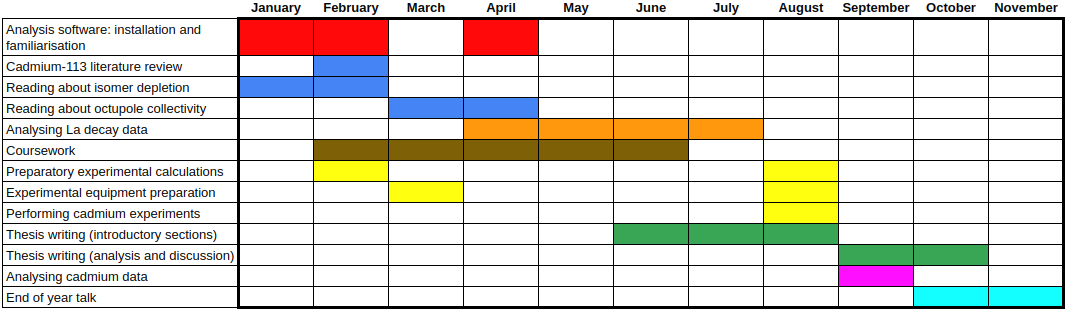
\includegraphics[width=\textwidth]{gantt}
	\caption{Planned timeline for this project. The inclusion of experimental preparation and execution in August represents the latest feasible time when this can occur. Tasks assigned to January through March have been completed. Tasks assigned to April are well underway.}
\label{fig:gantt}
\end{figure}
% room to tweak this for sure

\medskip
\noindent
The time allocated to each of the following steps is outlined in Figure~\ref{fig:gantt}.
The following data processing steps are central to the completion of a satisfactory project and will be performed using ROOT and Radware.
\begin{enumerate}
\item Check the energy and time calibration of the existing gamma ray data. % in progress.
\item Analyse the data in ROOT to construct a level scheme for $\ce{^{148,150,152}Ce}$.
\item Establish excitation energies and lifetimes of excited states in $\ce{^{148,150,152}Ce}$.
\item Identify the multipolarities and transitions between excited states of $\ce{^{148,150,152}Ce}$ to assess the degree of octupole collectivity present.
\item Measure the lifetimes of the $\ce{^{148,150,152}La}$ ground states and constrain their spin-parities (stretch goal).
\end{enumerate}
%Write introduction, motivation, background and methodology sections of thesis. I expect to finish these by August 31.

\medskip
\noindent
These analysis processes shall be continued in a dedicated manner until September 1 at the latest.
Concurrently, the introduction, motivation, background and methodology sections of the thesis shall be written.
As time progresses, we will continue to assess the feasibility of completing the planned $\ce{^{113}Cd}$ experiments before September 1.
This date is the latest feasible point at which there will remain time for thorough data analysis, collation of results and completion of the thesis.

\medskip
\noindent
If restrictions on access to the required experimental facilities are lifted by August 1, then the steps below will be executed. The exact timing will depend on beamtime being secured. All the steps below are essential unless otherwise specified.
%Dates somewhat arbitrary right now
\begin{enumerate}
\item Cool HPGe gamma-ray detectors to their operating temperatures using liquid nitrogen.
\item Perform STROP calculations to identify the optimal target thickness, taking into consideration the energies identified as optimal for maximising $\ce{^{113}Cd}$ yield.
\item Test HPGe detectors using PIXIE. Having had experience performing this process, the completion of this step will not take long.
\item Prepare $\ce{^{110}Pd}$ targets and create a mounting system for them. Establish whether we have enough targets and beamtime to perform experiments using both $\ce{^{7}Li}$ and $\ce{^{9}Be}$ beams.
\item Build the CAESAR array, in collaboration with A. J. Mitchell, Greg Lane, James Pope and other members of the Nuclear Spectroscopy group.
\item Perform experiments.
If the amount of beam time and/or targets is limited, only one of $\ce{^{7}Li}$ or $\ce{^{9}Be}$ may be used over a narrowed energy range.
\item Analyse data to construct a level scheme for $\ce{^{113}Cd}$ and identify any viable depletion pathways.
Deduce all possible spectroscopic information.
The analysis skills gained during the octupole collectivity part of the project will enable this to be completed efficiently.
\item Measure reaction cross sections as a function of energy.
%At a minimum, brief tests would be performed as part of step 6.
\item Investigate charged-particle-$\gamma$ coincidence data to identify beam-breakup reactions and measure their cross sections as a function of energy (stretch goal).
\item Pen and publish any significant results (stretch goal).
\item Write results, discussion and conclusion sections of the thesis, by October 29.
\item Prepare the final presentation, due November 5.
\end{enumerate}
This structure ensures that a satisfactory thesis will be generated.
But, as it is the busiest possible timeline with all possible parts included, it provides plenty of room to omit aspects should the time no longer be available for them.
At a bare minimum, new information on the neutron-rich isotopes $\ce{^{148,150,152}Ce}$ will be produced and significant skills in the analysis of multi-parameter nuclear data will be developed, achieving the two primary goals of this project.


%\vspace*{-\baselineskip}
%\def\bibfont{\small}
\bibliographystyle{ieeetr}
\bibliography{references.bib}{}
% No more than 20 refs


\end{document}